\documentclass[14pt,a4paper]{extarticle}

% ---- Кодировка и язык ----
\usepackage[utf8]{inputenc}
\usepackage[T2A]{fontenc}
\usepackage[russian]{babel}

% ---- Шрифт Times New Roman ----
\usepackage{mathptmx}
\usepackage{times}

% ---- Поля страницы ----
\usepackage[left=30mm, right=15mm, top=20mm, bottom=20mm]{geometry}

% ---- Межстрочный интервал 1.5 ----
\usepackage{setspace}
\onehalfspacing

% ---- Выравнивание по ширине, красная строка ----
\usepackage{indentfirst}
\setlength{\parindent}{1.25cm}

% ---- Математика ----
\usepackage{amsmath}
\usepackage{amssymb}

% ---- Таблицы ----
\usepackage{booktabs}
\usepackage{array}

% ---- Графика ----
\usepackage{graphicx}
\usepackage{float}

% ---- Подписи к рисункам ----
\usepackage{caption}
\captionsetup{
    labelsep=period,
    justification=centering,
    font={normalsize},
    skip=6pt
}

% ---- Оглавление ----
\usepackage{tocloft}
\renewcommand{\cftsecfont}{\normalfont}
\renewcommand{\cftsecpagefont}{\normalfont}
\renewcommand{\cftsubsecfont}{\normalfont}
\renewcommand{\cftsubsecpagefont}{\normalfont}
\setlength{\cftbeforesecskip}{4pt}
\renewcommand{\contentsname}{Содержание}

% ---- Гиперссылки ----
\usepackage[hidelinks]{hyperref}

% ---- Нумерация страниц ----
\usepackage{fancyhdr}
\pagestyle{fancy}
\fancyhf{}
\fancyfoot[C]{\thepage}
\renewcommand{\headrulewidth}{0pt}

\sloppy

% ================================================================
\begin{document}

% ---- Оглавление ----
\tableofcontents
\newpage

% ================================================================
\section{Универсальное множество лингвистической переменной}

Лингвистическая переменная <<Дерево (высота)>> формально описывается
пятёркой $\langle \beta,\, E,\, T,\, G,\, M \rangle$, где:

\begin{itemize}
    \item $\beta$ --- наименование лингвистической переменной: <<Дерево (высота)>>;
    \item $E$ --- универсальное множество (УМ);
    \item $T$ --- базовое терм-множество;
    \item $G$ --- синтаксическая процедура образования новых термов;
    \item $M$ --- семантическая процедура, ставящая каждому терму в соответствие
    нечёткое подмножество УМ~$E$.
\end{itemize}

Универсальное множество определяется как диапазон реальных высот деревьев
(от карликовых и декоративных форм до крупных лесных пород):

\begin{equation}
    \boxed{X = E = [0;\;50] \text{ м}}
\end{equation}

\noindent
\textbf{Обоснование:} нижняя граница --- 0~м (саженец, карликовое дерево),
верхняя граница --- 50~м (высокие деревья: дуб, ель, сосна).
Данный диапазон охватывает практически все виды деревьев умеренного климата.

% ================================================================
\section{Нечёткие множества для базовых термов}

Базовое терм-множество содержит четыре значения:

\begin{equation}
    T = \{\text{<<миниатюрное>>},\;\text{<<низкое>>},\;
          \text{<<среднее>>},\;\text{<<высокое>>}\}
\end{equation}

Каждому терму ставится в соответствие нечёткое подмножество~$A_i$
универсального множества~$E = [0;\,50]$~м с функцией принадлежности
$\mu_{A_i}(x) \in [0;\,1]$.
Все четыре НМ являются \textbf{нормальными} ($\sup \mu_{A_i}(x) = 1$)
и попарно перекрывающимися, что обеспечивает непрерывное покрытие УМ.

\begin{table}[H]
    \centering
    \caption{Границы базовых нечётких множеств}
    \begin{tabular}{lcccc}
        \toprule
        \textbf{Терм} &
        \textbf{Начало носителя} &
        \textbf{Лев.~точка перехода} &
        \textbf{Ядро} &
        \textbf{Прав.~точка перехода} \\
        \midrule
        $A_1$ --- миниатюрное & 0 м   & ---    & [0;\,5] м  & 7{,}5 м \\
        $A_2$ --- низкое      & 5 м   & 10 м   & 15 м       & 20 м    \\
        $A_3$ --- среднее     & 15 м  & 20 м   & 25 м       & 30 м    \\
        $A_4$ --- высокое     & 25 м  & 30 м   & [35;\,50] м & ---    \\
        \bottomrule
    \end{tabular}
\end{table}

\subsection{НМ \texorpdfstring{$A_1$}{A1} --- <<миниатюрное>>}

Левосторонняя трапециевидная функция принадлежности (убывающая):

\begin{equation}
    \mu_{A_1}(x) =
    \begin{cases}
        1, & x \leq 5, \\[4pt]
        \dfrac{10 - x}{5}, & 5 < x \leq 10, \\[8pt]
        0, & x > 10.
    \end{cases}
\end{equation}

\noindent
Носитель: $S_{A_1} = [0;\,10)$~м.
Ядро: $\operatorname{kernel} A_1 = [0;\,5]$~м.
Точка перехода: $\operatorname{pt} A_1 = \{7{,}5 \text{ м}\}$.

\subsection{НМ \texorpdfstring{$A_2$}{A2} --- <<низкое>>}

Треугольная функция принадлежности:

\begin{equation}
    \mu_{A_2}(x) =
    \begin{cases}
        0, & x \leq 5, \\[4pt]
        \dfrac{x - 5}{10}, & 5 < x \leq 15, \\[8pt]
        \dfrac{25 - x}{10}, & 15 < x \leq 25, \\[8pt]
        0, & x > 25.
    \end{cases}
\end{equation}

\noindent
Носитель: $S_{A_2} = (5;\,25)$~м.
Ядро: $\operatorname{kernel} A_2 = \{15 \text{ м}\}$.
Точки перехода: $\operatorname{pt} A_2 = \{10 \text{ м};\;20 \text{ м}\}$.

\subsection{НМ \texorpdfstring{$A_3$}{A3} --- <<среднее>>}

Треугольная симметричная функция принадлежности:

\begin{equation}
    \mu_{A_3}(x) =
    \begin{cases}
        0, & x \leq 15, \\[4pt]
        \dfrac{x - 15}{10}, & 15 < x \leq 25, \\[8pt]
        \dfrac{35 - x}{10}, & 25 < x \leq 35, \\[8pt]
        0, & x > 35.
    \end{cases}
\end{equation}

\noindent
Носитель: $S_{A_3} = (15;\,35)$~м.
Ядро: $\operatorname{kernel} A_3 = \{25 \text{ м}\}$.
Точки перехода: $\operatorname{pt} A_3 = \{20 \text{ м};\;30 \text{ м}\}$.

\subsection{НМ \texorpdfstring{$A_4$}{A4} --- <<высокое>>}

Правосторонняя трапециевидная функция принадлежности (возрастающая):

\begin{equation}
    \mu_{A_4}(x) =
    \begin{cases}
        0, & x \leq 25, \\[4pt]
        \dfrac{x - 25}{10}, & 25 < x \leq 35, \\[8pt]
        1, & x > 35.
    \end{cases}
\end{equation}

\noindent
Носитель: $S_{A_4} = (25;\,50]$~м.
Ядро: $\operatorname{kernel} A_4 = [35;\,50]$~м.
Точка перехода: $\operatorname{pt} A_4 = \{30 \text{ м}\}$.

\vspace{0.5em}
\noindent
График всех четырёх базовых нечётких множеств представлен на рис.~1.

\begin{figure}[H]
    \centering
    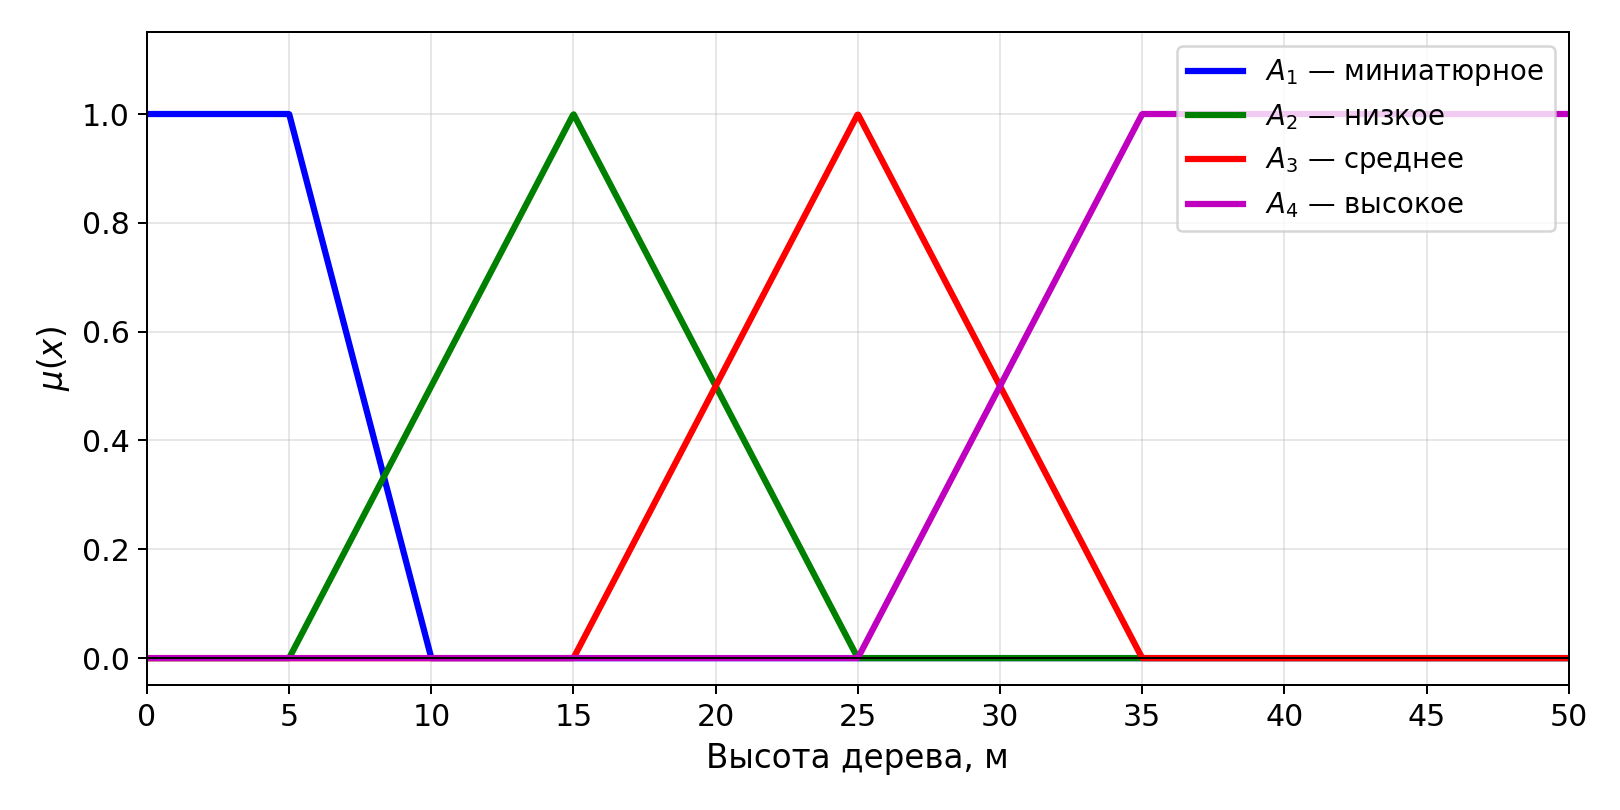
\includegraphics[width=0.90\textwidth]{fig1_base.png}
    \caption{Базовые нечёткие множества ЛП <<Дерево (высота)>>:
             $A_1$~--- <<миниатюрное>>, $A_2$~--- <<низкое>>,
             $A_3$~--- <<среднее>>, $A_4$~--- <<высокое>>}
    \label{fig:base}
\end{figure}

% ================================================================
\section{Параметры НМ <<среднее>>}

Для нечёткого множества $A_3$ --- <<среднее>> определим три характеристики.

\subsection{Носитель}

Носитель НМ~$A_3$ --- чёткое подмножество УМ~$E$,
включающее все элементы с ненулевой степенью принадлежности:

\begin{equation}
    S_{A_3} = \operatorname{supp} A_3
            = \{x \mid \mu_{A_3}(x) > 0\}
            = (15;\;35) \text{ м}
\end{equation}

\subsection{Точки перехода}

Точки перехода --- элементы $x \in E$,
для которых $\mu_{A_3}(x) = 0{,}5$:

\begin{itemize}
    \item Левый склон ($15 < x \leq 25$):
    \[
        \frac{x - 15}{10} = 0{,}5 \;\Rightarrow\; x = 20 \text{ м}
    \]
    \item Правый склон ($25 < x \leq 35$):
    \[
        \frac{35 - x}{10} = 0{,}5 \;\Rightarrow\; x = 30 \text{ м}
    \]
\end{itemize}

\begin{equation}
    \boxed{\operatorname{pt} A_3 = \{20 \text{ м};\;30 \text{ м}\}}
\end{equation}

\subsection{Ядро}

\begin{equation}
    \operatorname{kernel} A_3
    = \{x \mid \mu_{A_3}(x) = 1\}
    = \{25 \text{ м}\}
\end{equation}

НМ является \textbf{унимодальным}: степень принадлежности равна~1
лишь в единственной точке $x = 25$~м.

\subsection{Сводная таблица параметров}

\begin{table}[H]
    \centering
    \caption{Параметры НМ $A_3$ --- <<среднее>>}
    \begin{tabular}{lc}
        \toprule
        \textbf{Параметр} & \textbf{Значение} \\
        \midrule
        Носитель $S_{A_3}$                     & $(15 \text{ м};\;35 \text{ м})$ \\
        Точки перехода $\operatorname{pt} A_3$ & $\{20 \text{ м};\;30 \text{ м}\}$ \\
        Ядро $\operatorname{kernel} A_3$       & $\{25 \text{ м}\}$ \\
        Высота $h$                             & $1$ (нормальное НМ) \\
        \bottomrule
    \end{tabular}
\end{table}

\noindent
Графическая иллюстрация НМ <<среднее>> с отмеченными параметрами
представлена на рис.~2.

\begin{figure}[H]
    \centering
    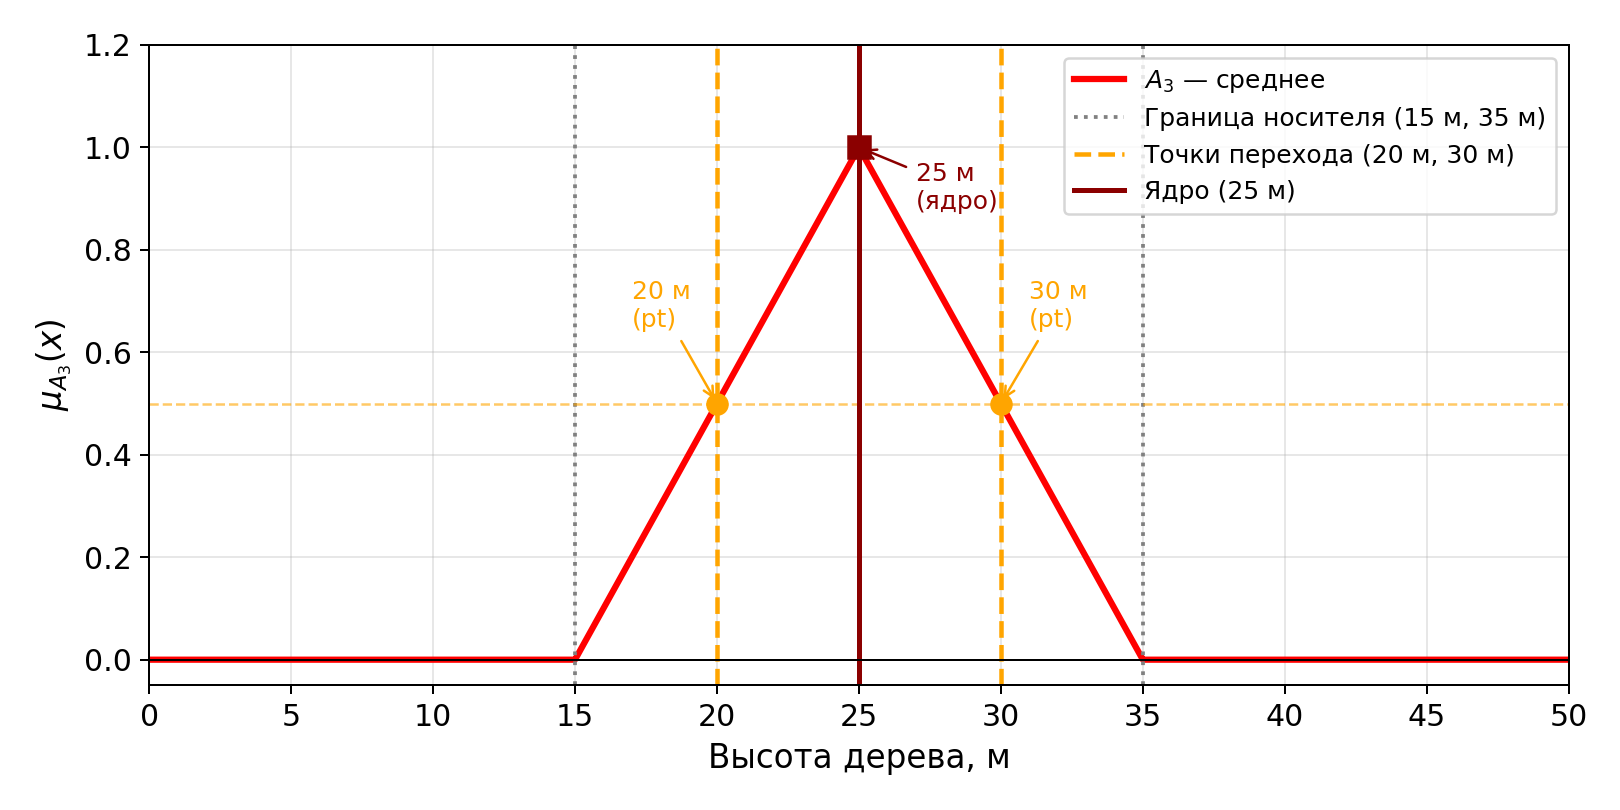
\includegraphics[width=0.90\textwidth]{fig2_srednie.png}
    \caption{НМ $A_3$ --- <<среднее>>: носитель $(15;\,35)$~м,
             точки перехода $\{20;\,30\}$~м, ядро $\{25\}$~м}
    \label{fig:srednie}
\end{figure}

% ================================================================
\section{Производные нечёткие множества}

Производные термы формируются с помощью синтаксической процедуры~$G$.
Семантическая процедура~$M$ сопоставляет каждой лингвистической операции
соответствующую операцию над НМ:

\begin{itemize}
    \item <<не>> --- дополнение:
          $\mu_{\bar{A}}(x) = 1 - \mu_A(x)$;
    \item <<или>> --- объединение:
          $\mu_{A \cup B}(x) = \max\!\left(\mu_A(x),\,\mu_B(x)\right)$;
    \item <<очень>> --- концентрирование:
          $\mu_{\mathrm{CON}(A)}(x) = \bigl[\mu_A(x)\bigr]^2$.
\end{itemize}

\subsection{<<Не миниатюрное>> ---
\texorpdfstring{$\overline{A_1}$}{}}

\textbf{Применяемая операция:} дополнение.

\begin{equation}
    \mu_{\overline{A_1}}(x) = 1 - \mu_{A_1}(x) =
    \begin{cases}
        0, & x \leq 5, \\[4pt]
        \dfrac{x - 5}{5}, & 5 < x \leq 10, \\[8pt]
        1, & x > 10.
    \end{cases}
\end{equation}

\noindent
\textbf{Вид:} возрастающая левосторонняя ФП с правым плато на уровне~1.
Все деревья выше~10~м полностью не являются миниатюрными ($\mu = 1$).

\noindent
График представлен на рис.~3.

\begin{figure}[H]
    \centering
    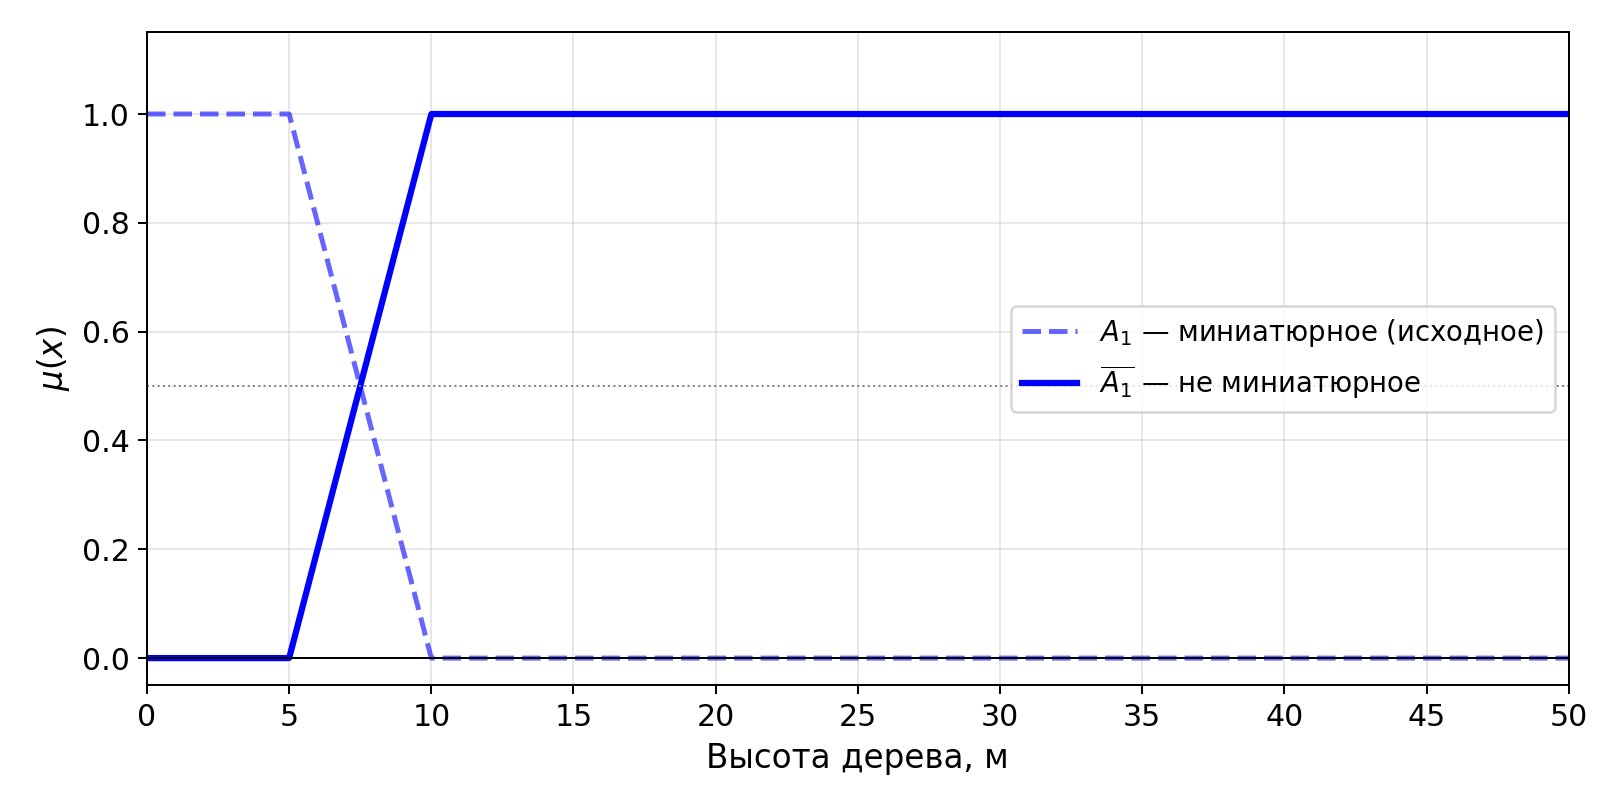
\includegraphics[width=0.90\textwidth]{fig3_not_mini.png}
    \caption{Производный терм <<не миниатюрное>> ($\overline{A_1}$):
             сплошная линия --- $\overline{A_1}$,
             пунктир --- исходное $A_1$}
    \label{fig:not_mini}
\end{figure}

\subsection{<<Миниатюрное или не низкое>> ---
\texorpdfstring{$A_1 \cup \overline{A_2}$}{}}

\textbf{Применяемые операции:} дополнение, затем объединение.

\noindent
\textbf{Шаг~1.} Строим $\overline{A_2}$ (<<не низкое>>):

\begin{equation}
    \mu_{\overline{A_2}}(x) = 1 - \mu_{A_2}(x) =
    \begin{cases}
        1, & x \leq 5, \\[4pt]
        \dfrac{15 - x}{10}, & 5 < x \leq 15, \\[8pt]
        \dfrac{x - 15}{10}, & 15 < x \leq 25, \\[8pt]
        1, & x > 25.
    \end{cases}
\end{equation}

\noindent
\textbf{Шаг~2.} Объединяем с $A_1$:

\begin{equation}
    \mu_{A_1 \cup \overline{A_2}}(x) =
    \max\!\left(\mu_{A_1}(x),\;\mu_{\overline{A_2}}(x)\right)
\end{equation}

\begin{table}[H]
    \centering
    \caption{Вычисление $\mu_{A_1 \cup \overline{A_2}}(x)$ по диапазонам}
    \begin{tabular}{lccc}
        \toprule
        \textbf{Диапазон} $x$ &
        $\mu_{A_1}(x)$ &
        $\mu_{\overline{A_2}}(x)$ &
        $\max(\cdot)$ \\
        \midrule
        $x \leq 5$        & $1$               & $1$               & $1$ \\
        $5 < x \leq 10$   & $\frac{10-x}{5}$  & $\frac{15-x}{10}$ & $\frac{10-x}{5}$ \\
        $10 < x \leq 15$  & $0$               & $\frac{15-x}{10}$ & $\frac{15-x}{10}$ \\
        $15 < x \leq 25$  & $0$               & $\frac{x-15}{10}$ & $\frac{x-15}{10}$ \\
        $x > 25$          & $0$               & $1$               & $1$ \\
        \bottomrule
    \end{tabular}
\end{table}

\noindent
\textbf{Вид:} НМ с двумя областями полного членства ($x \leq 5$~м и $x > 25$~м)
и провалом в диапазоне $5\text{--}25$~м.

\noindent
График представлен на рис.~4.

\begin{figure}[H]
    \centering
    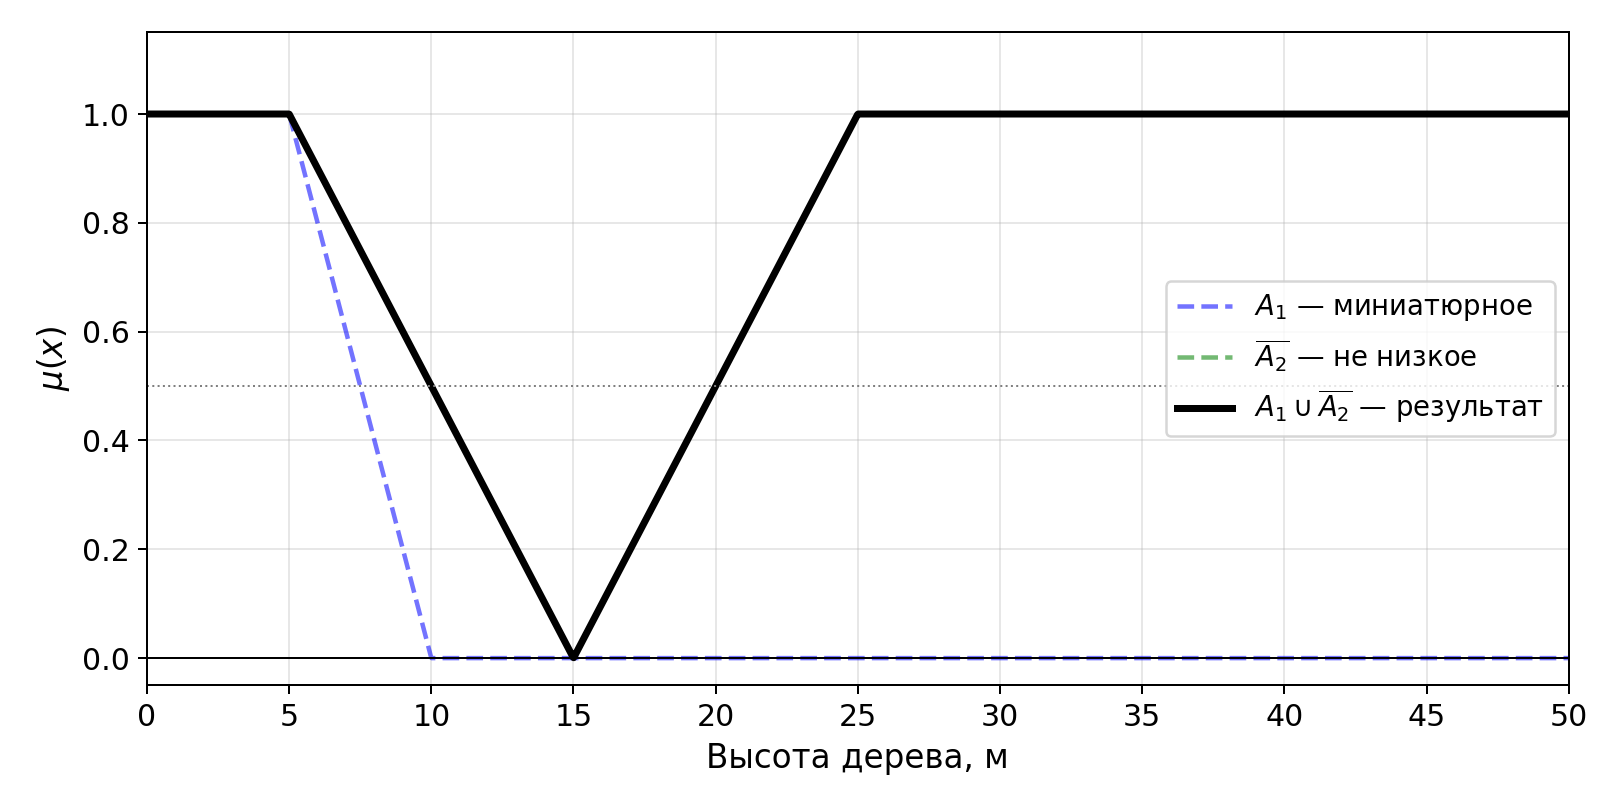
\includegraphics[width=0.90\textwidth]{fig4_mini_or_not_low.png}
    \caption{Производный терм <<миниатюрное или не низкое>>
             ($A_1 \cup \overline{A_2}$):
             сплошная линия --- результат,
             пунктир --- исходные $A_1$ и $\overline{A_2}$}
    \label{fig:mini_or_not_low}
\end{figure}

\subsection{<<Очень высокое>> ---
\texorpdfstring{$\mathrm{CON}(A_4) = A_4^2$}{}}

\textbf{Применяемая операция:} концентрирование ($\alpha = 2$).

\begin{equation}
    \mu_{\mathrm{CON}(A_4)}(x) = \bigl[\mu_{A_4}(x)\bigr]^2 =
    \begin{cases}
        0, & x \leq 25, \\[4pt]
        \left(\dfrac{x - 25}{10}\right)^{\!2}, & 25 < x \leq 35, \\[10pt]
        1, & x > 35.
    \end{cases}
\end{equation}

\noindent
\textbf{Вид:} правосторонняя ФП с выпуклым (медленным) нарастанием ---
кривая лежит ниже исходной $A_4$ на всём переходном участке $[25;\,35]$~м,
что соответствует более строгому критерию высоты.

\noindent
График представлен на рис.~5.

\begin{figure}[H]
    \centering
    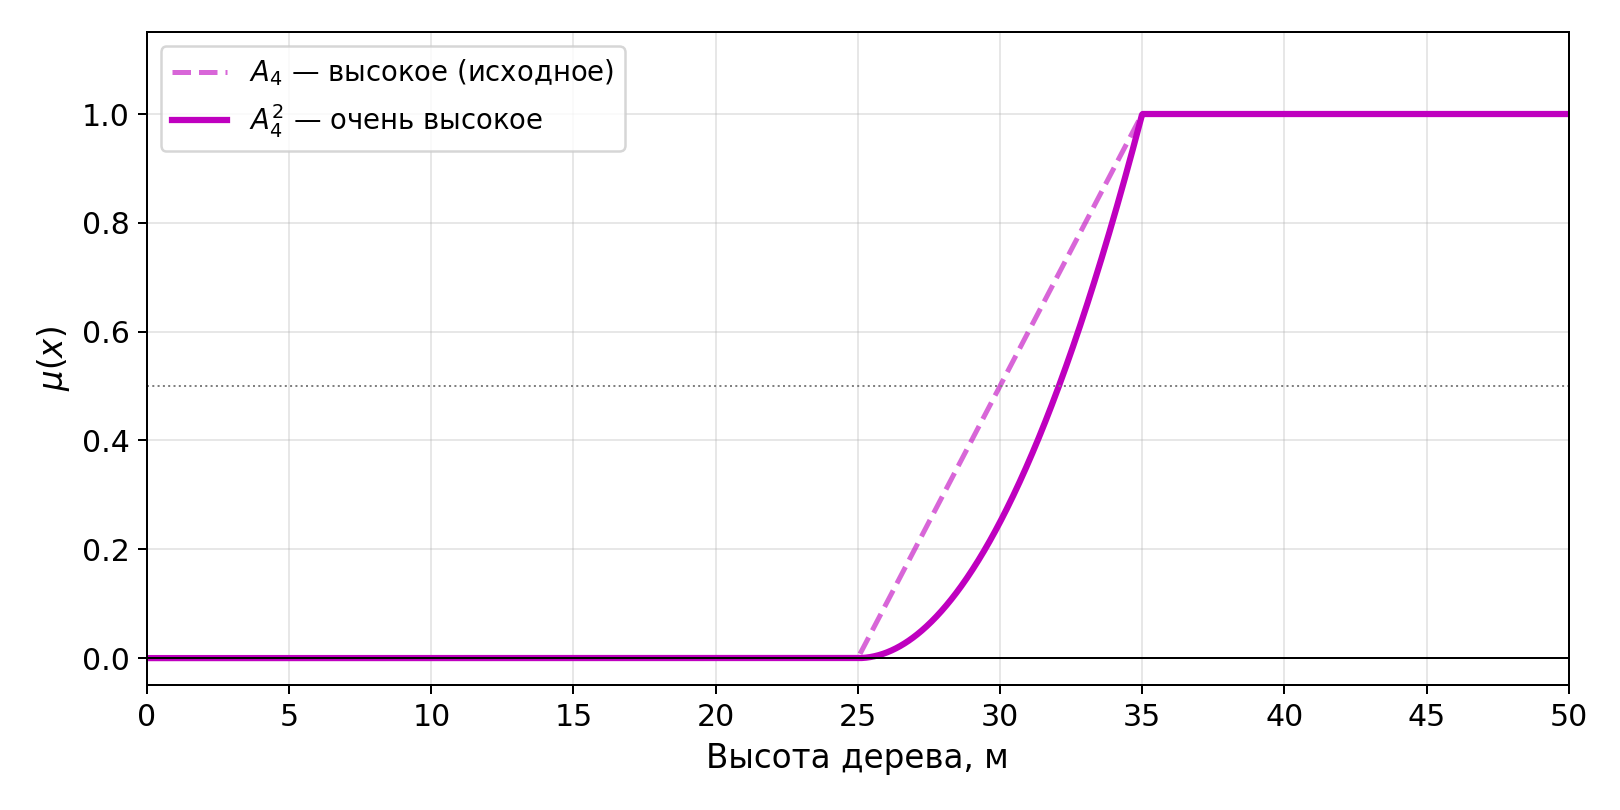
\includegraphics[width=0.90\textwidth]{fig5_very_high.png}
    \caption{Производный терм <<очень высокое>>
             ($\mathrm{CON}(A_4) = A_4^2$):
             сплошная линия --- $A_4^2$,
             пунктир --- исходное $A_4$}
    \label{fig:very_high}
\end{figure}

\subsection{<<Низкое или среднее>> ---
\texorpdfstring{$A_2 \cup A_3$}{}}

\textbf{Применяемая операция:} объединение.

\begin{equation}
    \mu_{A_2 \cup A_3}(x) =
    \max\!\left(\mu_{A_2}(x),\;\mu_{A_3}(x)\right)
\end{equation}

\begin{table}[H]
    \centering
    \caption{Вычисление $\mu_{A_2 \cup A_3}(x)$ по диапазонам}
    \begin{tabular}{lccc}
        \toprule
        \textbf{Диапазон} $x$ &
        $\mu_{A_2}(x)$ &
        $\mu_{A_3}(x)$ &
        $\max(\cdot)$ \\
        \midrule
        $x \leq 5$         & $0$               & $0$               & $0$ \\
        $5 < x \leq 15$    & $\frac{x-5}{10}$  & $0$               & $\frac{x-5}{10}$ \\
        $15 < x \leq 20$   & $\frac{25-x}{10}$ & $\frac{x-15}{10}$ & $\frac{25-x}{10}$ \\
        $x = 20$           & $0{,}5$           & $0{,}5$           & $0{,}5$ \\
        $20 < x \leq 25$   & $\frac{25-x}{10}$ & $\frac{x-15}{10}$ & $\frac{x-15}{10}$ \\
        $25 < x \leq 35$   & $0$               & $\frac{35-x}{10}$ & $\frac{35-x}{10}$ \\
        $x > 35$           & $0$               & $0$               & $0$ \\
        \bottomrule
    \end{tabular}
\end{table}

\noindent
\textbf{Вид:} широкий купол от~5~м до~35~м с двумя вершинами $\mu = 1$
в точках $x = 15$~м и $x = 25$~м, и седлом $\mu = 0{,}5$ в точке $x = 20$~м.

\noindent
График представлен на рис.~6.

\begin{figure}[H]
    \centering
    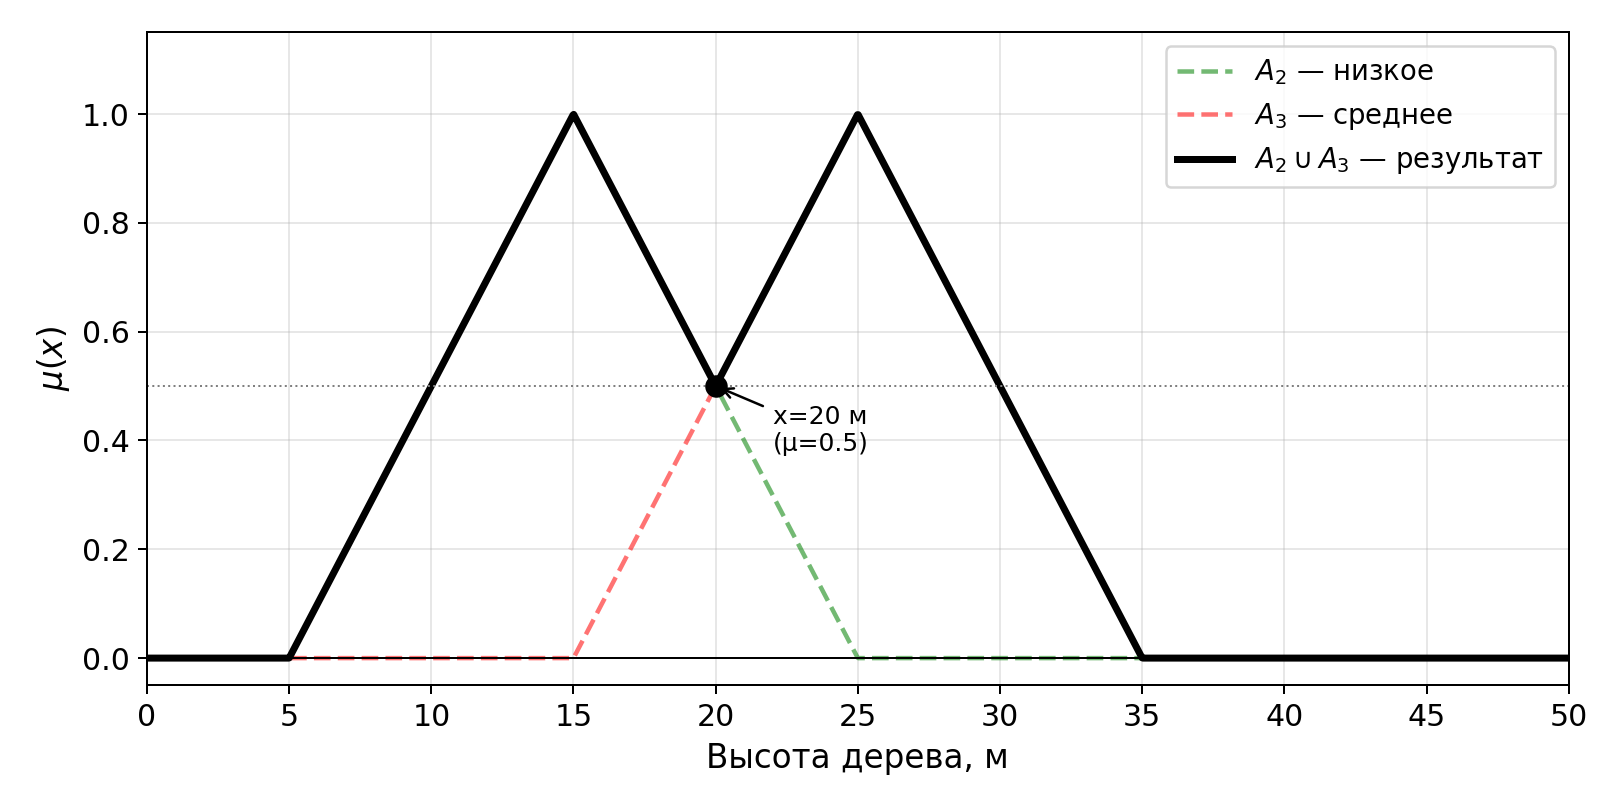
\includegraphics[width=0.90\textwidth]{fig6_low_or_mid.png}
    \caption{Производный терм <<низкое или среднее>> ($A_2 \cup A_3$):
             сплошная линия --- результат,
             пунктир --- исходные $A_2$ и $A_3$}
    \label{fig:low_or_mid}
\end{figure}

% ================================================================
\section{Итоговая сводка}

\begin{table}[H]
    \centering
    \caption{Сводная таблица по всем заданиям}
    \begin{tabular}{p{4.2cm} p{3.8cm} p{5.5cm}}
        \toprule
        \textbf{Терм} & \textbf{Операция} & \textbf{Формула ФП} \\
        \midrule
        \multicolumn{3}{l}{\textit{Базовые термы}} \\
        Миниатюрное ($A_1$) & ---
            & Лев.~трапеция, $[0;\,10)$~м \\
        Низкое ($A_2$)      & ---
            & Треугольник, $(5;\,25)$~м \\
        Среднее ($A_3$)     & ---
            & Треугольник, $(15;\,35)$~м \\
        Высокое ($A_4$)     & ---
            & Прав.~трапеция, $(25;\,50]$~м \\
        \midrule
        \multicolumn{3}{l}{\textit{Производные термы}} \\
        Не миниатюрное
            & Дополнение
            & $\mu = 1 - \mu_{A_1}(x)$ \\
        Миниатюрное или не низкое
            & Дополнение~+ объединение
            & $\mu = \max(\mu_{A_1}(x),\,1 - \mu_{A_2}(x))$ \\
        Очень высокое
            & Концентрирование ($\alpha = 2$)
            & $\mu = [\mu_{A_4}(x)]^2$ \\
        Низкое или среднее
            & Объединение
            & $\mu = \max(\mu_{A_2}(x),\,\mu_{A_3}(x))$ \\
        \bottomrule
    \end{tabular}
\end{table}

\end{document}